% 双生子佯谬
% 双生子悖论|孪生子悖论

% 基本完成
\pentry{斜坐标系表示洛伦兹变换\upref{SROb}}

双生子佯谬,又称孪生子佯谬,是一个著名的相对论问题.“佯谬”一词的意思是“看起来像是错误但实际上不是”,其中“谬”指“错误”,而“佯”指“假的”.它曾经被认为是一个悖论,但在今天已经被完美解决了,所以成了一个佯谬.和\textbf{时间的变换与钟慢效应}\upref{SRtime}词条的结尾所指出的一样,我们将从双生子佯谬入手,尝试讨论非惯性系眼中的时空.

\subsection{问题描述}

假设地球在某个惯性系$K_1$中静止,忽略一切引力等作用,把地球考虑成一个质点.为方便理解,也可以说$K_1$是“地球系”.在地球上有一对完全同龄的双胞胎,其中弟弟始终留在地球上,而哥哥则乘坐飞船离开地球.称飞船的参考系$K_2$是“飞船系”,同样看成一个质点.一段时间以哥哥返回并降落在地球上.称飞船的参考系$K_2$是“飞船系”.当飞船降落后,兄弟俩的年龄是否有差异?差异是什么?

\subsection{双生子佯谬的解答}

我们现有的工具只有狭义相对论,而弟弟所在的地球系是一个惯性系,因此我们可以先从地球系开始讨论.假设兄弟俩各戴着一只完美的手表,走时绝无误差,并且双方都把飞船出发的一刻设为时间零点.这样,我们只需要比较哥哥返回地球时两人手表的读数即可.

问题的最简形式,就是哥哥以匀速直线运动离开地球,某一时刻瞬间反向,沿着原道路以相反速度回到地球.这样,我们甚至不需要关心飞船降落的过程,因为当飞船和地球重合的时候,它们的时空坐标完全相同,被认为是同一个事件,无论在哪个参考系看来都是同时发生的,不会出现同时性的相对性.这样,无论飞船有没有和地球保持静止,我们都可以比较哥哥和弟弟各自手上的手表读数.

事实上并不会存在这样瞬间反向的运动,那么这个模型有物理意义吗?答案是有的,我们只需要耍一个小小的花招.

考虑两艘飞船,都在哥哥的航道上,一艘自地球出发做匀速直线运动,另一艘飞船自远方飞向地球,速度和第一艘相反.这样,两艘飞船都是惯性系,都可以用我们已有的狭义相对论方法去讨论它们眼中的时空.这两艘飞船的运动可以看成是,飞船$1$始终离开地球,飞船$2$先靠近地球,然后穿过地球,即两艘飞船一直匀速,只是中途重合了一瞬间;但是也可以看成,飞船$1$离开地球后,到达重合点突然变成飞船$2$,飞向地球;飞船$2$也在重合点处突然变成飞船$1$,飞离地球.为了把这个双飞船的模型等价转化为问题中单飞船的情况,我们只需要让两艘飞船对表,使得它们重合时手表读数相同,然后只观察“飞船$1$飞到重合点后变成飞船$2$再回到地球”这一过程就可以,将“飞船$2$飞到重合点后变成飞船$1$再飞向无穷远”这一过程视为\textbf{不存在}.

\subsubsection{坐标网格与等时线划分}

\begin{figure}[ht]
\centering
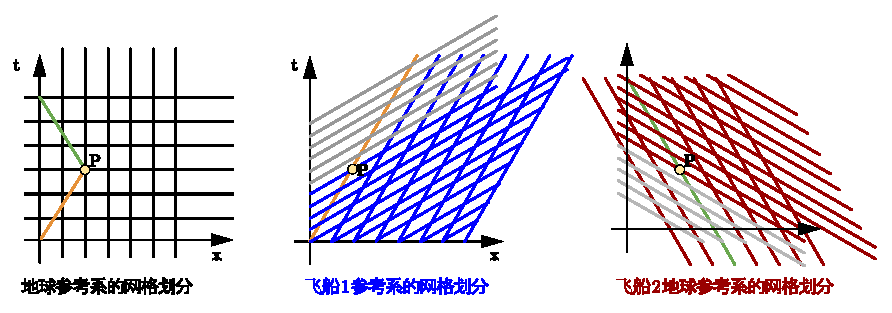
\includegraphics[width=14cm]{./figures/Twins_1.pdf}
\caption{在\textbf{地球系}中所看到的三个惯性系的网格划分.} \label{Twins_fig1}
\end{figure}

我们将地球、飞船$1$和飞船$2$的坐标网格分别表示如\autoref{Twins_fig1} ,三个网格都是在\textbf{地球系}中划分的.图中的点$P$表示“飞船$1$和飞船$2$相互转换”这一事件.显然,地球系自身的等时线都和$x$轴平行,等距线都和$t$轴平行,因此它的网格看起来是一个矩形划分,如图中左边的黑色网格所示;飞船$1$的坐标网格如中间的蓝色划分,其中橙色线代表空间坐标始终为$0$的点,即飞船$1$本身的轨迹,而灰色线代表忽略掉的等时线,因为它们出现在$P$点之后,是不存在的;飞船$2$的坐标网格如右边的红色划分,其中绿色线代表空间坐标始终为$0$的点,即飞船$2$本身的轨迹,而灰色线同样代表忽略掉的等时线,因为出现在$P$之前,不存在.

\autoref{Twins_fig1} 没有明显画出来的是,各等距线被灰色等时线所覆盖的部分也要忽略掉.

现在,把两个飞船的坐标网格放到一起,擦掉各自被忽略掉的等时线和等距线部分,就得到了飞船系在整个运动过程中的等时线划分,如\autoref{Twins_fig2} 所示:

\begin{figure}[ht]
\centering
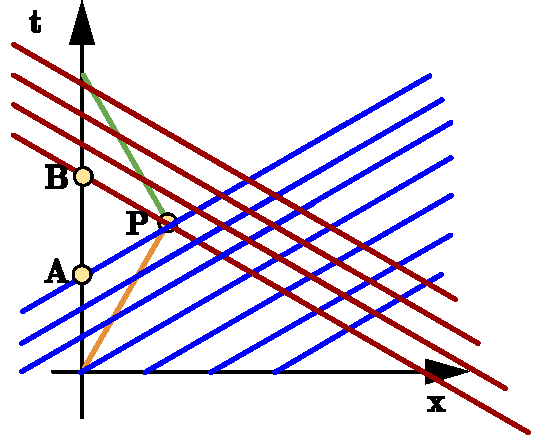
\includegraphics[width=10cm]{./figures/Twins_2.pdf}
\caption{飞船系的等时线划分.} \label{Twins_fig2}
\end{figure}

\subsubsection{地球系眼中的飞船时间流逝}

在地球上的弟弟看来,尽管飞船的速度在$P$点处突然反向,但是大小是不变的,因此飞船上的时间流速一直都是地球上时间流速的$\sqrt{1-v^2}$倍,其中$v$是指飞船的速度大小.如果飞船回到地球的一瞬间,弟弟的手表显示时间是$t_0$的话,那么哥哥的手表显示的时间应该是$t_0\sqrt{1-v^2}$.

\subsubsection{飞船系眼中的地球时间流逝}

在飞船上的哥哥看来,地球上的时间流速应该是飞船上时间流速的$\sqrt{1-v^2}$倍,其中$v$是指地球的速度大小,和地球眼中飞船的速度大小是相等的.但是和地球不同的是,在飞船反向的那一刻,即事件$P$处,有两条等时线,分别和$t$轴相交于$A$点和$B$点.也就是说,在飞船看来,$A$和$B$是同时发生的事件,甚至由于它们到飞船的距离也一样,因此在飞船看来是同一个事件.

$A$事件和$B$事件分别代表弟弟的手表在地球上显示$t_1$和$t_2$,其中$t_1<t_2<t_0$.也就是说,在飞船上的哥哥看来,当飞船突然变向的时候,地球上的弟弟的手表显示的时间瞬间从$t_1$跳到了$t_2$.整体上,哥哥眼中弟弟的时间流逝速度还是比飞船慢的,但是在飞船变向时弟弟的时间突然跃变了一下,所以导致最终二人相遇时,弟弟手表的读数还是大于哥哥的.

\begin{exercise}{}\label{Twins_exe1}
假设二人再次相遇时,弟弟的手表显示时间为$t_0$.计算在地球系中$A$和$B$的时间差$\Delta t$.
\end{exercise}

\autoref{Twins_exe1} 的计算结果应为$\Delta t=v^2t_0$.如果代入地球系计算的结果,即在哥哥看来整个飞行过程持续时间为$t_0\sqrt{1-v^2}$,那么飞船系中弟弟的时间流速只有哥哥的$\sqrt{1-v^2}$倍,因此弟弟的时间应该连续流逝了$t_0\sqrt{1-v^2}\sqrt{1-v^2}=t_0(1-v^2)$;加上弟弟的时间有$\Delta t=v^2t_0$的跃变,因此在哥哥看来,相遇时弟弟的手表读数是$\Delta t_0+t_0(1-v^2)=t_0$,与地球系中计算的结果相同.

\subsubsection{解答总结}

当哥哥不在地球上时,读表的同时性是相对的,一方眼中的同时读表,在另一方看来就是一先一后的,不是同时.因此兄弟俩如果要比较彼此的手表读数,就得见一次面,因为见面属于同一事件(时空坐标完全相同),无论在哪个参考系看来都是同时的,见面时的两人手表的读数是绝对的,这时候的比较才有意义.但是双方要再次见面,哥哥就不可避免地要经历变速过程.如果是瞬间变速,那么在哥哥看来弟弟的手表读数会在变速的一瞬间跃变,导致最终还是具有更大的读数.因此当两人见面时,无论在谁看来都是弟弟的时间流逝更多,因此弟弟的年龄应该比哥哥大.

实际情况中我们不可能观测到对方的手表读数跃变,因为我们不可能瞬间变速,而是要经历一个加速过程.加速过程可以看成无数匀速过程相加\footnote{严格来说,可以把加速过程分成$n$段匀速过程,研究其中各事件的时空坐标,再取$\lim\limits_{n\rightarrow\infty}$的极限就得到加速过程中各事件的时空坐标.},在加速过程中每一个时空点的瞬时自身系中观察地球的时空坐标,那么我们会发现在加速过程中,哥哥眼中弟弟的时间流逝速度会大大加快,导致最终相遇时总的时间流逝还是弟弟更多.

\subsection{思考}

在\autoref{Twins_fig2} 中$P$的右侧有一块锥形区域,其中每个点都经过了一红一蓝两个等时线,这意味着什么?

如果在某个比$P$点距离地球更远的地方是火星,其中火星、地球和飞船始终保持在一条直线上(理想地),火星上有一个人也拿着手表在计时.在整个飞行过程中,从飞船系看,火星上这个人的手表读数是如何变化的?







